\section{Model Training: \namel}

\subsection{Injecting Legal Knowledge}

To address the limitations of legal knowledge inherent in the base LLaMa model, we adopted a continued pretraining (CPT) strategy utilizing a comprehensive Indian legal corpus. For this purpose, we selected the LLaMa2-7B architecture \cite{touvron2023llama}, which features a substantial context length of 2K, allowing for effective handling of legal texts. This choice facilitates a direct comparison with previous state-of-the-art results on the PredEx dataset \cite{nigam2024legaljudgmentreimaginedpredex}. This approach significantly enhances the model's understanding and relevance within the Indian legal framework, thereby improving its predictive capabilities and application in legal tasks.

\subsection{Learning Reasoning Skills}

To further develop the model's reasoning skills, particularly for legal prediction and explanation tasks, we conducted supervised finetuning (SFT) using data from specific downstream tasks. This dataset includes case decisions along with their corresponding explanations, all annotated by legal experts. The fine-tuning process was crucial for enhancing the model's ability to understand and apply legal principles effectively, bridging the gap between general knowledge and the specialized requirements of legal reasoning tasks. This focused fine-tuning was pivotal in improving the model's performance in real-world legal scenarios.

However, the fine-tuning of such models typically demands substantial computational resources and extensive training data. Given the constraints of limited computational power and the specific nature of our legal task-related dataset, we prioritized efficient training methods to optimize both computational costs and data usage. We employed parameter-efficient tuning techniques, such as the Low-Rank Adaptation (LoRA) method \cite{hu2021lora}, to fine-tune the LLaMa-2 7B model. This approach enabled us to maximize the utility of available data and minimize the need for extensive computational resources, ensuring a cost-effective yet powerful fine-tuning process for developing \texttt{\namel}.

%%%%%%%%%%%%%%%%%%%%%%%%%%%%%%%%%%%%
\begin{figure*}[t] % [h] specifies the placement of the figure InLegalLlama_flow_7.drawio.pdf -> InLegalLlama_flow_Arnab_sir_version.pdf ->InLegalLlama_flow (1).drawio.pdf->InLegalLlama_flow_final_Coloured_Enlarged_Figure.drawio.pdf
    \centering % Centers the figure
    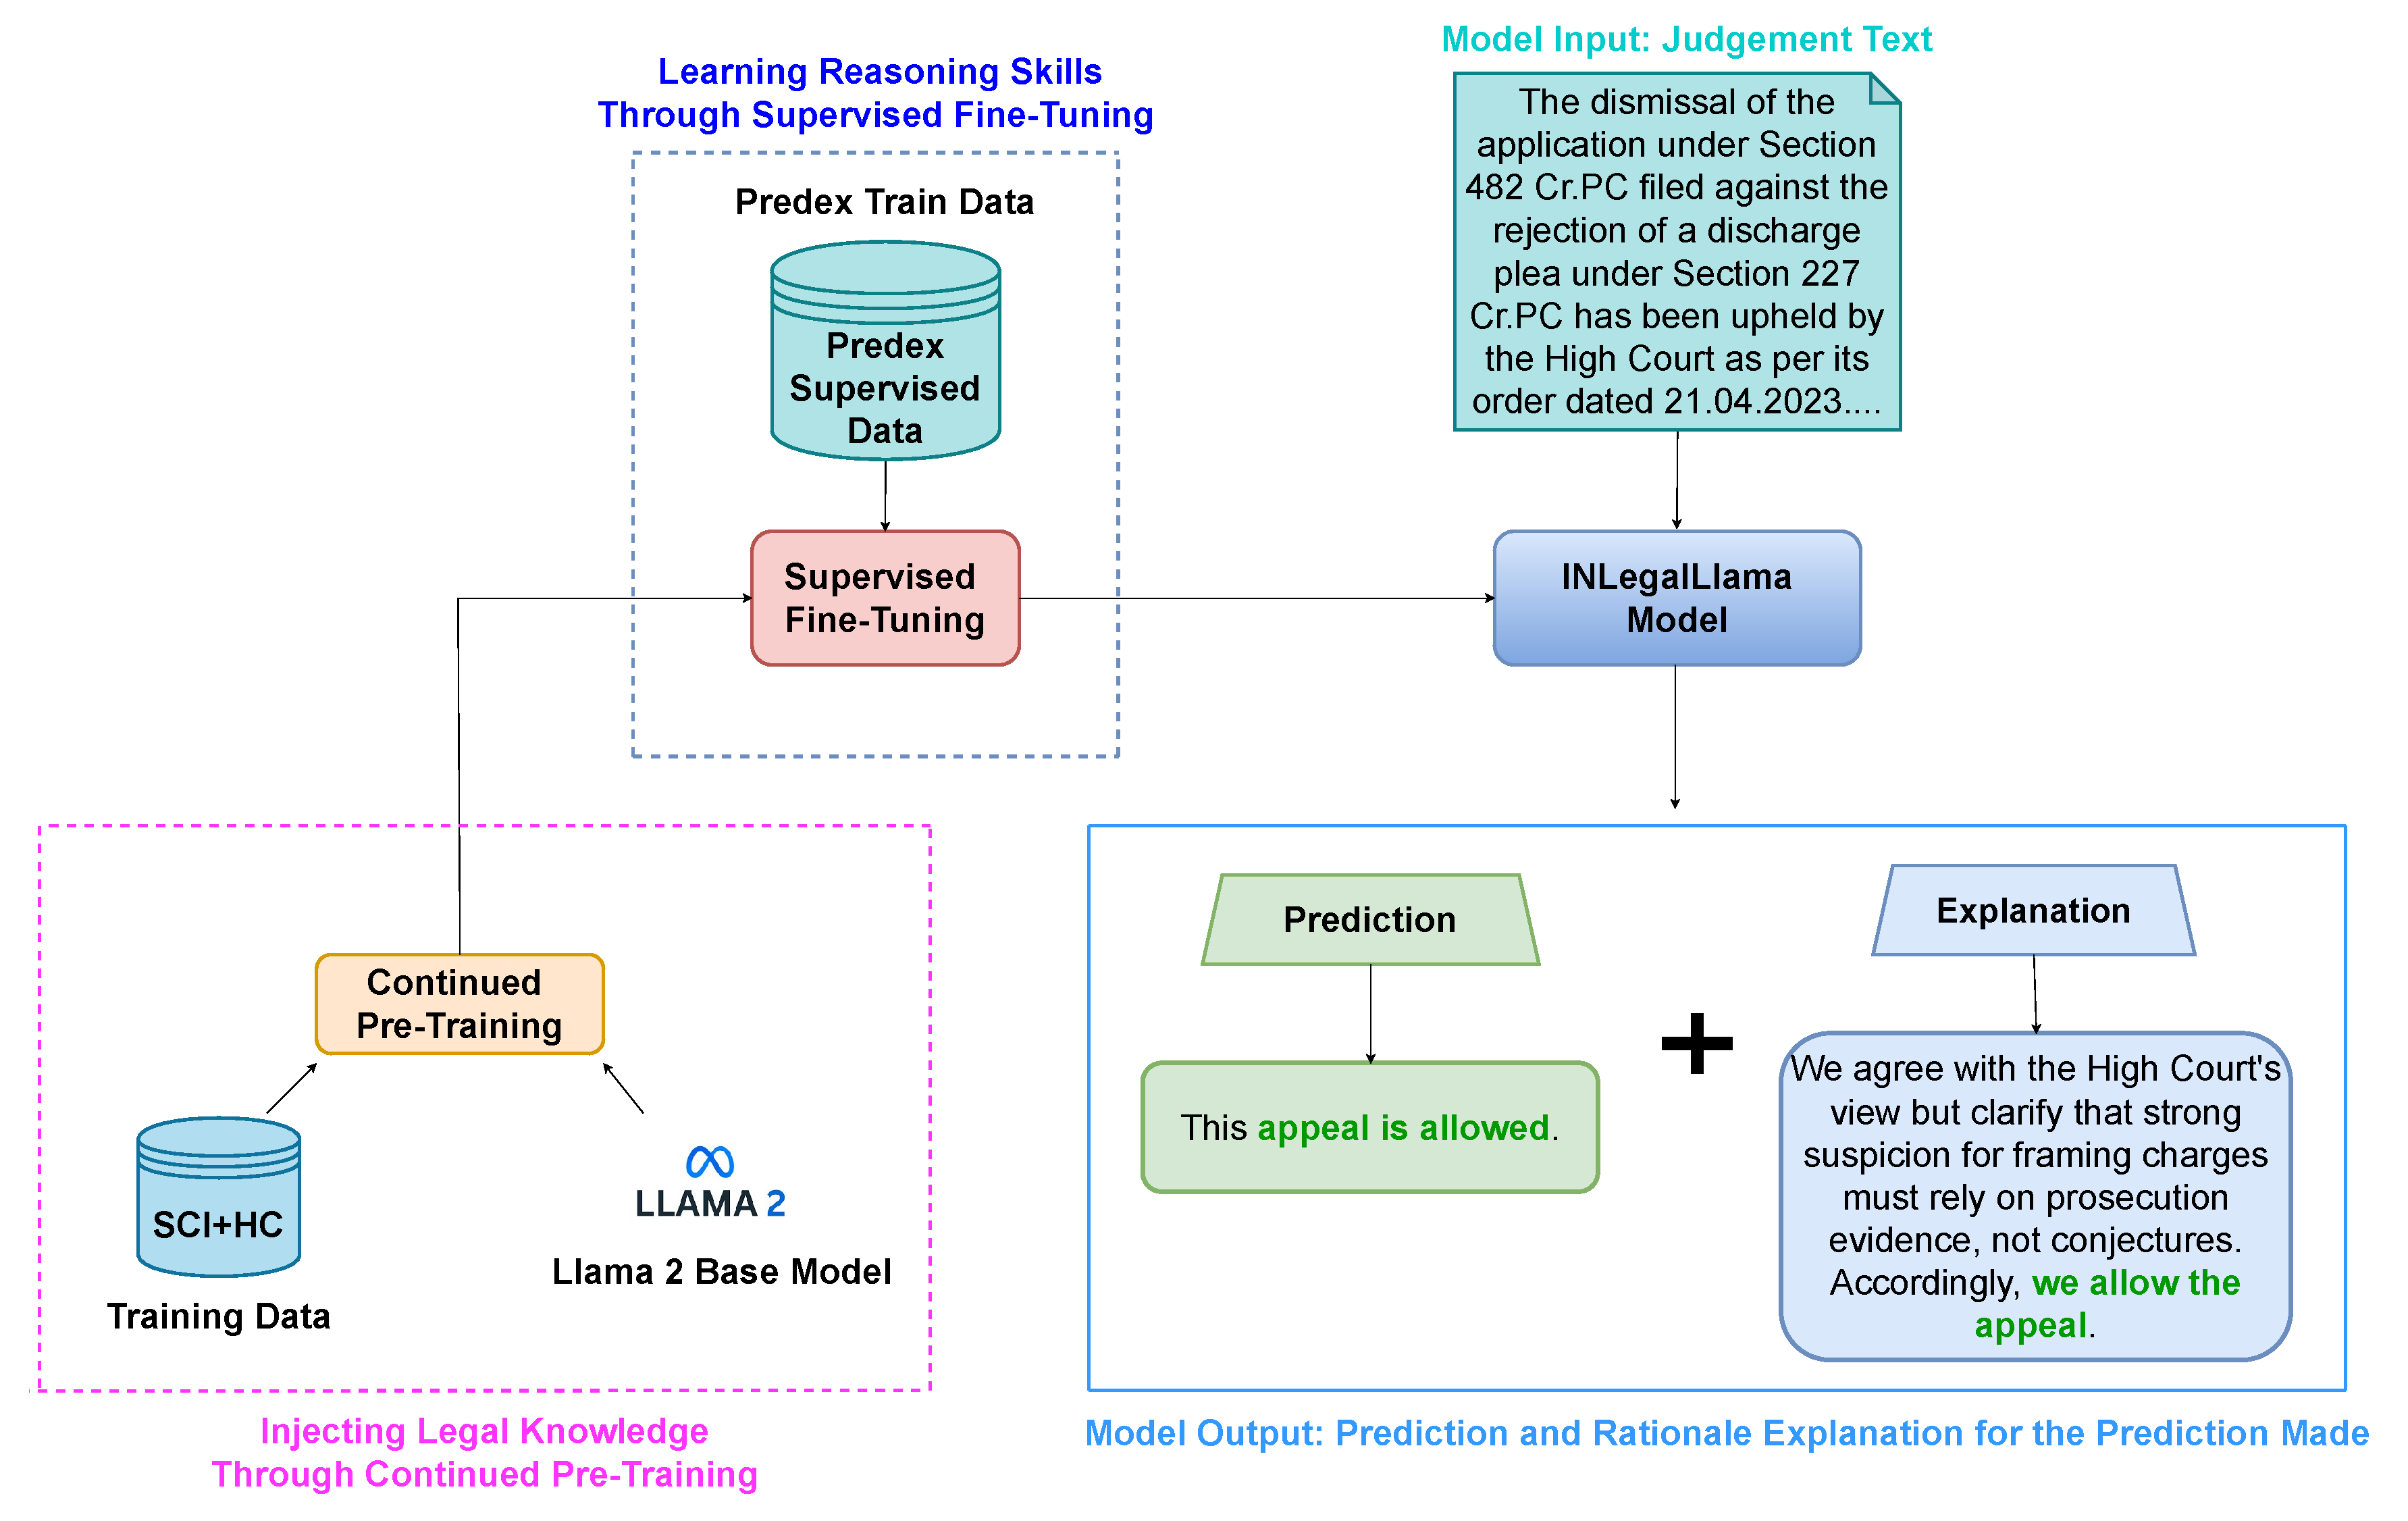
\includegraphics[width= \linewidth]{figures/InLegalLlama_flow_final_Coloured_Enlarged_Figure.drawio.pdf} 
    \caption{\namel flow diagram}
    \label{fig:InLegalLlama-Flow-Diagram} % For referencing the figure
\end{figure*}
%%%%%%%%%%%%%%%%%%%%%%%%%%%%%%%%%%%%
